\documentclass[11pt,letterpaper]{article}
\usepackage[utf8]{inputenc}

%----- Configuración del estilo del documento------%
\usepackage{epsfig,graphicx}
\usepackage[left=2cm,right=2cm,top=1.8cm,bottom=2.3cm]{geometry}
\usepackage{fancyhdr}
\usepackage{lastpage}

\usepackage{xcolor}
\usepackage{soul}
\newcommand{\mathcolorbox}[2]{\colorbox{#1}{$\displaystyle #2$}}

%------ Paquetes para demostraciónes y árboles de derivación ------%
\usepackage{bussproofs}
\usepackage{scalefnt}

%Color bibi
\definecolor{bibi}{RGB}{0,103,148}
% Otros colores

% ------ Paquetes para arboles --------%
\usepackage{bussproofs}

\usepackage{cite}
\usepackage{multicol}
\setlength{\columnsep}{1.5cm}
\setlength{\columnseprule}{.5pt}

\pagestyle{fancy}
\fancyhf{}
\rfoot{\textit{Página \thepage \hspace{1pt} de \pageref{LastPage}}}

%------ Paquetes matemáticos básicos --------%
\usepackage{amsmath}
\usepackage{amssymb}
\usepackage{amsthm}

%------ Paquetes para codigo --------%
\usepackage{verbatim}
\usepackage{listings}
\lstset{language=Haskell, basicstyle=\ttfamily, keywordstyle=\color{blue}, commentstyle=\color{gray}, stringstyle=\color{green}}

\usepackage{tikz}


\begin{document}

%------ Encabezado -------- %
\begin{center}
    \begin{minipage}{3cm}
    	\begin{center}
    		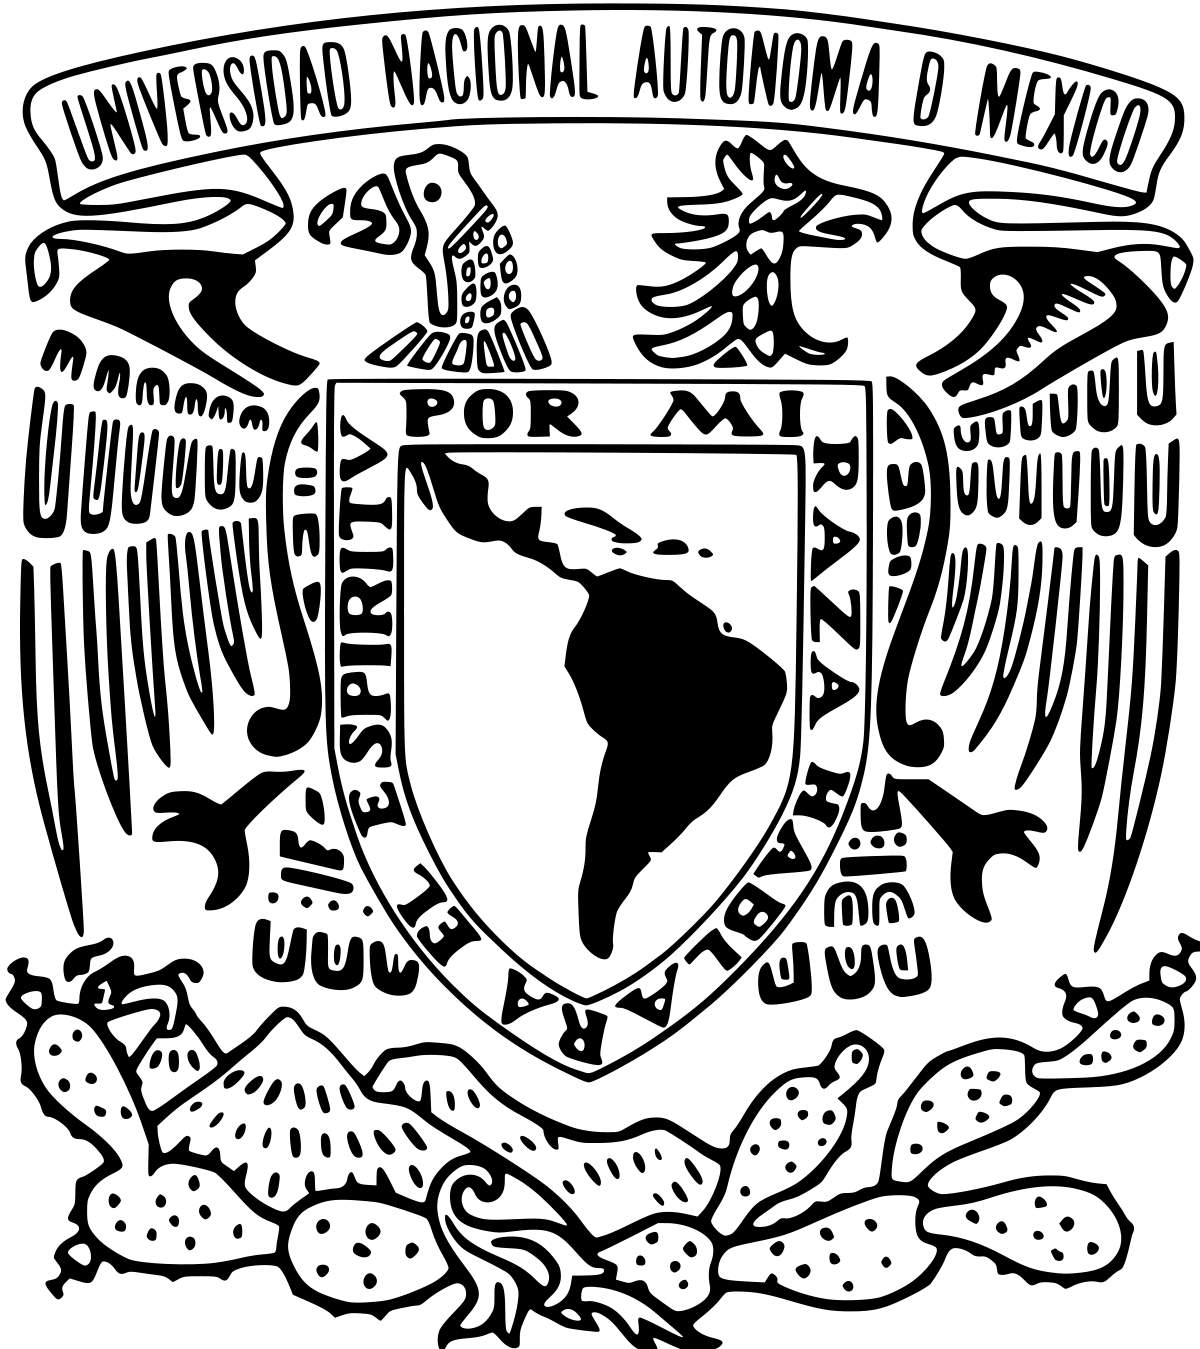
\includegraphics[height=3.2cm]{src/Img/Logo_UNAM.png}
    	\end{center}
    \end{minipage}\hfill
    \begin{minipage}{10cm}
    	\begin{center}
    	\textbf{\large Universidad Nacional Autónoma de México}\\[0.1cm]
        \textbf{Facultad de Ciencias}\\[0.1cm]
        \textbf{Inteligencia Artificial $|$ 7003}\\[0.1cm]
        Examen Parcial 1 $|$ Introducción y Agentes \\[0.1cm]
        Sosa Romo Juan Mario $|$ 320051926 \\[0.1cm]
        24/02/24
    	\end{center}
    \end{minipage}\hfill
    \begin{minipage}{3cm}
    	\begin{center}
    		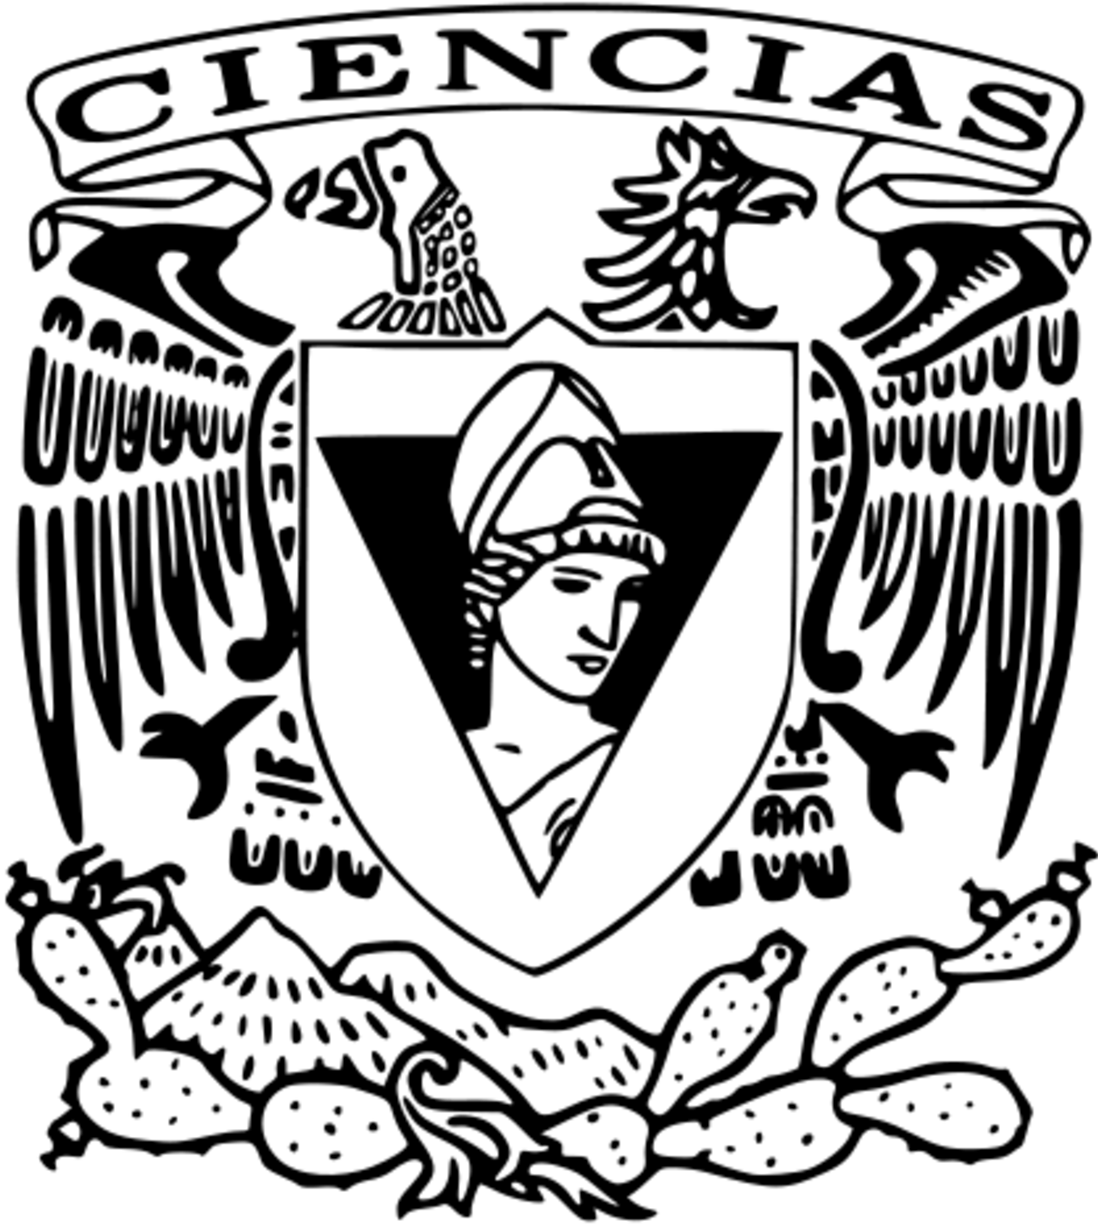
\includegraphics[height=3.2cm]{src/Img/Logo_FC.png}
    	\end{center}
    \end{minipage}
\end{center}


\rule{16.9cm}{0.1mm}
\vspace{0.3cm}

\vspace{0.3cm}
%------ Ejercicios -------- %
\begin{enumerate}
    \item \textbf{Ejercicio 1.} (25 pts.) Evalúa las siguientes expresiones usando las téctnicas de paso de prámetros que se indican. En cada caso debes mostrar cómo queda el ambiente y memoria final, tal y como se vio en clase. \vspace{0.3cm}

\begin{itemize}
    \item Evalúa el siguiente código bajo paso por valor y por referencia.
\begin{lstlisting}
(let [(list1 (box '(1 2 3)))
    (list2 (box '(4 5 6)))
    (concat-lists (lambda (x y)
                    (begin
                        (set! x (append (unbox x) (unbox y)))
                        (set! y '(0)))))]
    (begin
        (concat-lists list1 list2)
        (list (unbox list1) (unbox list2))))
\end{lstlisting}

    \item Evalúa el siguiente código bajo paso por nombre y por necesidad.
\begin{lstlisting}
(let [(acc 0)
    (conditional (lambda (x)
                    (if (> x 0)
                        (begin (set! acc (+ acc 1)) acc)
                        (begin (set! acc (- acc 1)) acc))))
    (compute (lambda (y) (* y y)))]
(compute (conditional acc)))
\end{lstlisting}
\end{itemize}



    
    \item \textbf{Explica los tres paradigmas principales de la I.A., así como sus características principales (1 pt.).}

\begin{itemize}
    \item \textbf{Simbólico}
    
    En esencia, este enfoque busca conseguir "inteligencia" mediante el uso de símbolos y reglas. Es útil si queremos hacer cosas más determinísticas o más estructuradas. \vspace{.3cm}

    Es un enfoque más limitado en términos de escalabilidad, pues se tiene que, de cierta forma, saber de manera previa lo que se quiere que el sistema sepa. \vspace{.3cm}
    
    \cite{russell2020artificial}

    \item \textbf{Estadístico}
    
    Como su nombre lo indica, este paradigma se apoya en métodos probabilísticos y estadísticos, como la regresión, para intentar corregir o determinar la incertidumbre. Incluye métodos como los de aprendizaje supervisado, no supervisado y de refuerzo. \vspace{.3cm}

    En sí, son bastante útiles para detectar patrones en grandes cantidades de datos y se aplican en modelos económicos o en los conocidos algoritmos de redes sociales. \vspace{.3cm}

    En esencia, este enfoque presenta dos problemas principales. El primero, y el más grande (no solo para este tipo de IA), es la cantidad y calidad de los datos; al tratarse de modelos diseñados para procesar grandes volúmenes de información, conseguir datos y verificar que sean válidos es complicado. El segundo problema es el de la caja negra: a diferencia del enfoque anterior, en el que los procesos son relativamente más simples de entender y simular, en este paradigma, al no ser necesario mostrar o explicar cada paso sino solo el resultado y el modelo, se vuelve bastante más complejo comprender su funcionamiento. \vspace{.3cm}

    \cite{bishop2006pattern}

    \item \textbf{Neuronal}
    
    Finalmente, tenemos el paradigma neuronal. Como su nombre lo indica, esta corriente se basa en el funcionamiento de los cerebros orgánicos, especialmente el de los humanos; en su núcleo se plantea la idea de computar a través de una red de unidades independientes distribuidas, que reciben una serie de señales y generan otra serie de señales tras procesarlas. \vspace{.3cm}

    Además de las unidades, denominadas neuronas, existen capas de entrada, ocultas y de salida, que son agrupaciones de neuronas con comportamientos específicos. Una ventaja de este enfoque es que pierde gran parte de la estructura rígida que requieren los otros dos, volviéndose más flexible y permitiendo enfocarse en las entradas y salidas. Esto, a su vez, implica que nuevamente surge el problema de la caja negra, y en este caso, aún más marcado. \vspace{.3cm}

    Este enfoque es el más popular actualmente, a mi parecer, por su gran escalabilidad; además, estos modelos son capaces de tratar con datos no estructurados, lo que los hace mucho mejores en tareas de traducción o procesamiento de imágenes. \vspace{.3cm}

    \cite{goodfellow2016deep}
\end{itemize}

Finalmente, me gusta agregar que, aunque son tres enfoques diferentes, en la práctica es muy común utilizar una combinación para aprovechar las ventajas de cada uno y compensar las limitaciones de los otros.


    \item \textbf{Ejercicio 3.} (25 pts.) Realiza el juicio de tipo para cada una de las siguientes expresiones, usa las reglas vistas en clase o define una nueva regla en caso de ser necesario. Observa que la primera expresión no tiene anotaciones de tipo, por lo que tendras que definir las reglas para verificar los tipos. \vspace{0.3cm}

\begin{enumerate}
\item 
\begin{lstlisting}
(let (g (lambda (x) (x 4)))
    (g (lambda (y) (-y 2))))
\end{lstlisting}

\item 
\begin{lstlisting}
(letrec (f : number -> number
    (fun (x : number) : number
        (if0 x 1 (* n (f (- n 1))))))
    (f 5))
\end{lstlisting}
\end{enumerate}

    \item \textbf{Investiga y explica brevemente de qué se trata el juego de la imitación de Alan M. Turing. Cita tus fuentes (0.5 pt.).}

También conocido como la prueba de Turing, es un experimento mental propuesto por Alan M. Turing en su artículo \textit{Computing Machinery and Intelligence}. La idea es que, para probar la consciencia o su ausencia en las máquinas, se sitúan una máquina, una persona y una segunda persona que actuará como juez; de esta forma, mediante preguntas y respuestas, el mediador, representado en la figura 'C', debe determinar quién es la computadora y quién es la persona. Si el sistema es capaz de engañar a un alto porcentaje de los jueces, se le considera que ha pasado la prueba de Turing. \vspace{.3cm}

\cite{turing1950computing}

\begin{figure}[h]
    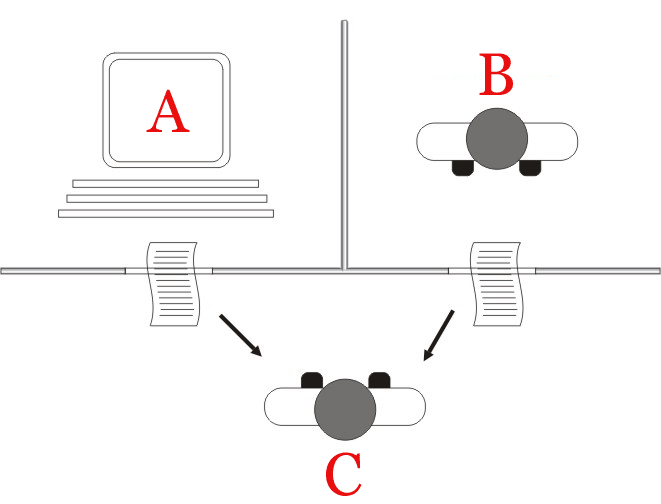
\includegraphics[width=10cm]{src/Img/Turing_test_diagram.png}
    \centering
    \caption{\cite{testTuring}}
\end{figure}

Aunque el hecho de que el sistema pase el test, en realidad, no nos indica más que su capacidad para comunicarse de manera coherente. Aun así, es altamente probable que nos encontremos ante un escenario similar al experimento del cuarto chino de John Searle, en el que la computadora realmente no tiene idea de lo que está haciendo, pero es capaz de engañar al mediador mediante tácticas inteligentes, generalmente basadas en métodos estadísticos y neuronales. \vspace{.3cm}

\end{enumerate}

\end{document}